%------------------------------------------------------------------------------
%	CAPITOLO 7
%------------------------------------------------------------------------------

\chapter{La Nuova Beccheria - Avviso}
\index[Personaggi]{Gioele}Gioele\footnote{\textbf{Gioele}, (ndr) quelli che l'hanno conosciuto, mi hanno raccontato che Gioele, o Giuele, stava seduto davanti ad un caffè dove dava dei pareri. Veniva pagato in natura, quindi con un salame o cose del genere.} calzolaio che aveva disertato da un pezzo il dischetto\footnote{Il dischetto era il tavolino usato dai calzolai nel loro lavoro} per vivere con le bricciole della rendita degli altri: pur di non fare nulla, si peccava di essere un superuomo, un grande elettore, causidico\footnote{Chi difendeva qualcuno in giudizio senza essere avvocato}, letterato. Di tutta l'arca della sua scienza aveva solo la miseria del letterato. S'intrufava\footnote{Intrufolava} ed era un assiduo degli spettacoli pubblici, come le prove dei cavalli sullo stradone, le cause in pretura, le adunanze\footnote{Riunioni comunali} al consiglio comunale, le baruffe in piazza, il montaggio e lo smontaggio dei baracconi dei saltimbanchi e cose di quanto può occorrere a chi non ha né arte né parte ad uno sfaccendato per ingannare il tempo ed emergere\footnote{[...]e tutto ciò che può servire ad uno sfaccendato, che non ha nessun lavoro, per passare il tempo.}.\\
\indent Un giorno gli si presenta \index[Personaggi]{Pagani Ettore (macellaio)}Ettore Pagani e lo prega di fargli un avviso al pubblico perché vuole aprire una nuova beccheria. \\
\indent Il nostro \index[Personaggi]{Gioele}Gioele trionfante, per l'onore e col miraggio forse del guadagno di una bracciola, si prende \index[Personaggi]{Pagani Ettore (macellaio)}Pagani e lo porta in farmacia, dove era di casa un po', e dove trovava gratis, carta, penna e calamaio e persone che l'attorniavano per ridere alle sue spalle.\\
\\
\indent Ecco l'Avviso:

\textcal{ \Huge
\vspace{-1cm}
\begin{center}
	Avviso
\end{center}
\begin{center}
	Nella bottega di \index[Personaggi]{Faccani Rodolfo (barbiere)}Faccani Rodolfo barbiere viene aperta una bottega di carne da bue.\\
\end{center}
\begin{center}
	d'avanti L 1 al Kg\\
	didietro L 1.20 al Kg
		\rightline{Pagani Ettore}
\end{center}
} \normalsize \normalfont 

\indent Letto forte a chiara voce, provocò risata.\\\\
\index[Personaggi]{Vincenzo della Borghina} Vincenzo della Borghina s'azzardò di dire: <<la carne di bue... è al fieno \footnote{(ndr) Dopo varie letture ed interpretazioni, non sono riuscito a trovare un senso a questa frase. Forse intendeva dire che la carne al fieno era pregiata e dire "didietro" la screditava.}>>\\
\indent\index[Personaggi]{Gioele}Gioele: <<Dam a qua e manifest. E poi imbezèl a vut ca dèga `carne da cul'?\footnote{<<Dammi qua il manifesto. E poi, imbecille, vuoi che dica `carne da culo'?}>>. \\
\indent Aspetta.\\
\indent Prese il manifesto corresse borbottando <<Sumàr a vit ac azonz `ora'\footnote{<<Somaro, vedi, aggiungo `ora'>>}>>
\newpage
\textcal{ \Huge
\begin{center}
	Avviso
\end{center}
\begin{center}
	Nella bottega di \index[Personaggi]{Faccani Rodolfo (barbiere)}Faccani Rodolfo barbiere viene aperta \underline{ora} una bottega di carne da bue.\\
\end{center}
\begin{center}
	d'avanti L 1 al Kg\\
	didietro L 1.20 al Kg\\
	\rightline{Pagani Ettore}
\end{center}
} \normalsize \normalfont
<<A vit ora cum ca deg. Portal a la stêpa e pu dì cu la fat Giuèla!\footnote{<<Vedi ora come dico. Portalo alla stampa e dì che l'ha fatto Gioele.>>}>>\\
\indent E così fu stampato e consacrato alle risate del pubblico.

 \begin{figure}[htb]
    \centering
    %\vspace{-0.7cm}
    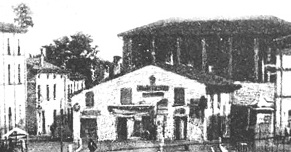
\includegraphics[width=\textwidth]{macelleria}
    \caption[Macelleria Pagani]{A sinistra il negozio di macelleria di \index[Personaggi]{Pagani Ettore (macellaio)}\textbf{Ettore Pagani} (padre di \index[Personaggi]{Pagani Armando}Armando Pagani, e' pcher, che dopo la guerra aveva il negozio sotto i portici del palazzo Grazioli) che ne continuò il mestiere fino agli anni '60, trasferendo il locale-macelleria sotto il porticato del \index[Luoghi]{Palazzo Grazioli}Palazzo Grazioli, a destra della casa Marini. Nel negozio dello spaccio avviò l'attività nel 1938 un altro macellaio: \index[Personaggi]{Marri Walter}Walter Marri, attivo fino agli anni '60 e poi trasferitosi sotto i portici di piazza Monti, dove a tutt'oggi esiste il suo locale gestito dal figlio, dopo la sua morte.\label{fig:macelleria}}
    %\vspace{-0.3cm}
\end{figure}






































%
